\documentclass[12pt,fleqn]{article}\usepackage{../common}

\begin{document}

Lineer Cebir - Ders 2

$$ x + 2y + z = 2 $$

$$ 3x + 8y + z = 12 $$

$$ 4y + z = 2 $$

Lineer sistem cozme zamani geldi. Cozum icin mesela determinantlari
kullanmayacagiz, bu konu ileride gelecek, ama eliminasyon metotu
kullanacagiz. Eliminasyon tum yazilim paketlerinin kullandigi cozum
metotudur. Eger basariya ulasirsa (ulasamayabilir de) o zaman sonucu bulmus
olur, ki cogunlukla da basarili olur. $A$ matrisi iyi huylu ise, basarili
olur, ki ustteki ornegimiz oyle. Tabii biz eliminasyon uygularken kendimize
bir yandan sunu soracagiz - hangi sartlarda bu islem basarisiz olurdu? Bu
soru ogretici olacak. 

Eliminasyon aslinda cok basit bir islemdir, sinifta olan sizler, bizler
bile bu metotu bulabilirdik. Gauss buldu bu yontemi tabii, cunku bizden
daha once dogmustu. 

Eliminasyonu tarif ederken bu islemleri matris operasyonlari olarak
gosterecegim [yani tum matrise etki eden turden cebirsel islemlerden
bahsediyor hoca], cunku dersimizdeki tum temel fikirler, sozler, laflar
olarak degil matris operasyonlari olarak gosterilecek. Bir operasyon mesela
bir matrisi carpmak. 

Ustteki ornege gelelim: bu sisteme tekabul eden $A$ matrisi, 

$$ 
\left[\begin{array}{rrr}
1 & 2 & 1 \\
3 & 8 & 1 \\
0 & 4 & 1
\end{array}\right]
 $$

Artik tum islemleri bu matris uzerinde yapabiliriz. Ilk bastaki esitlikler,
arti, vs gibi semboller iceren sembollere bakmiyoruz bile. Eliminasyonun
ihtiyaci olan tek sey artik ustteki $A$ matrisi. 

Eliminasyon ne yapar? Mesela ornek bir islem, 1. denklemi uygun bir sayiyla
carpmak, 2. satirdan cikarmak. Amac $x$'i disari atmak. Boylece denklemi ve
bilinmeyenleri azaltmis olacagiz. Carpan ne olmali? 

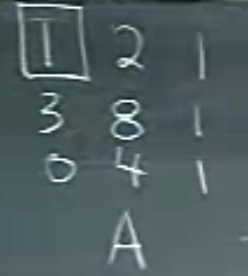
\includegraphics[height=4cm]{2_01.png}

1. satirda $x$ icin verilen katsayi '1' sayisini kullanacagim. Matrisin o
hucresini isaretledim, onu kullanacagimi belirtmek icin. Lineer cebirde
denir ki bu hucreyi 'pivot' olarak secmis oldum. Simdi eliminasyon islemini
yapalim; pivot satirini 3 ile carpip ikinciden cikartalim.

$$ 
\left[\begin{array}{rrr}
    1 & 2 & 1 \\
    0 & 2 & -2 \\
    0 & 4 & 1
  \end{array}\right]
$$

Peki bu arada esitligin sag tarafina, yani $b$'ye ne oldu? Degisimlerin ona
da yapilmasi lazim, bazi yazilim paketleri mesela Matlab sag tarafi
sonradan degistiriyor, ben de Matlab gibi olayip bari, degisimi sonradan
yapayim. 

Simdiye kadar ne yaptik? 2,1 kordinatindaki sayiyi ``temizlemis'' olduk,
sifir haline getirdik. Bundan sonra 3,1 kordinatina gidilecek, ama orasi
zaten sifir halinde; yani isleme gerek yok. 

Kalanlar nedir? Alttaki kisimdir,

$$ 
\left[\begin{array}{rrr}
    \dots & \dots & \dots \\
    \dots &  2 & -2 \\
    \dots & 4 &  1
  \end{array}\right]
$$

Iki ustteki matriste tek bir $x$ haricinde tum $x$'ler yokoldu, tek kalan
1. satirdaki $x$ ise zaten sonuc demektir. Ustteki durumda elimizde sadece
iki tane denklem kalmis gibidir artik, $x$ biliniyor. Bundan sonrasi
ozyineli (recursive) bir islem gibidir sanki, matris icinde daha ufak bir
matris bulduk, oradan daha ufak baska bir matrise gidecegiz, bu sirada
cozumleri teker teker bulacagiz.

Ikinci pivota ve onun satirina gidelim,

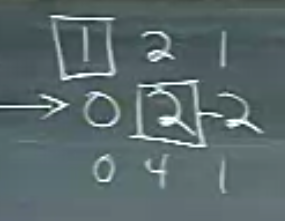
\includegraphics[height=4cm]{2_02.png}

Bunu yapmamizin amaci 4,2 kordinatindaki '4' sayisini temizlemek. 2. satiri
2 ile carpalim, 3. satirdan cikartalim,

$$ 
\left[\begin{array}{rrr}
1 & 2 & 1 \\
0 & 2 & -2 \\
0 & 0 & 5
\end{array}\right]
 $$

Bu matrise $U$ adini verecegim, bu harfi kullandim cunku ustteki matris bir
``ust-ucgensel (uppertriangular)'' matris. Eliminasyonun tum amaci bu
matrise ulasmaktir. Daha genel baglamda soylemek gerekirse bilimsel
hesaplama dunyasinin en temel, en yaygin islemi ustte gordugumuz,
yaptigimiz bu islemdir. Pek cok kisinin ``bu hesabi nasil daha hizli
yaparim'' diye dusunce sarfettigini, ugrastigini gorursunuz, cunku cok, cok
gerekli bir istir. 

Isleme donelim: pivot secerken sunu eklemek lazim, sifir pivot olsaydi o
pivot olarak secilmezdi. Ustteki durumda cikmadi ama ortaya cikabilirdi. 

Bu arada, ileriki derslere biraz atlama yapmak gerekirse, eger ustteki
matrisin eger determinantini hesaplamam gerekseydi pivotlari alip
birbiriyle carpmam yeterli olurdu. 

Simdi basarisizlik durumuna bakalim; ustteki islem hangi kosullarda
basarisiz olurdu? Eger 1,1 kordinatini pivot sectigim zaman orada bir sifir
olsaydi mesela.. Ne demistik? Sifir pivot olmaz. Peki bu durumda ne
yaparim? Basit bir numara, satir degis-tokusu yaparim, mesela en ustteki
satiri hemen altindaki ile degis-tokus yaparim, boylece sifir artik
caprazda yer almaz, ve baktigim satirdaki pivot artik sifir olmaz. Not: Bu
arada bir matriste satir degisimi yapmanin denklem sistemi icin hicbir
zarari yoktur, cunku ne de olsa her satir ayridir, her satir ayri bir
denkleme tekabul eder. Denklemlerin hangi sirada yazildigi onemli degil.

Fakat bazen kendimi kurtarmam mumkun olmayabilir, mesela eger matris su
halde olsaydi, 

$$ 
\left[\begin{array}{rrr}
1 & 2 & 1 \\
3 & 8 & 1 \\
0 & 4 & -4
\end{array}\right]
 $$

eliminasyon yapa yapa sona gelirdik, ve cikarma isleminden sonra $-4$
sifir olurdu. 

$$ 
\left[\begin{array}{rrr}
    \dots & \dots & \dots \\
    \dots &  2 & -2 \\
    \dots & 4 &  0
  \end{array}\right]
$$

Bu durumda kendimizi kurtaramazdik, cunku altta degis-tokus yapacak satir
bulamazdik. Boylece sifir pivot durumu ortaya cikardi, ve bu tersi
alinamayan matris isareti olurdu.

Neyse; biz basari durumundan devam edelim, artik tum bilinmeyenleri bulmak
icin geriye koyma (backsubstitution) yapabiliriz. Matlab ne yapardi? Biz ne
yapariz? Bir teknik, gecirme islemine baslamadan once $b$'yi alip $A$'ya
eklemlemek, 

$$ 
\left[\begin{array}{rrrr}
1 & 2 & 1 & 2\\
3 & 8 & 1 & 12 \\
0 & 4 & 1 & 2
\end{array}\right]
 $$

Bu bize eklemlenmis (augmented) yeni bir matris verir. Boylece $A$
uzerinde yaptigim her islemi otomatik olarak $b$ uzerinde yapmam
kolaylasir. Tum carpma-cikarma islemlerini eklemlenmis matris uzerinde de
uygularsam,

$$ 
\underbrace{
\left[\begin{array}{rrr}
1 & 2 & 1 \\
0 & 2 & -2 \\
0 & 0 & 5  
\end{array}\right.}_{U}
\underbrace{
\left. \begin{array}{r}
 2\\
 6\\
 -10 
\end{array}\right]}_{c}
 $$












\end{document}
